\documentclass{beamer}
\usetheme{Madrid}

\usepackage{biblatex}

\title{RFID Sicherheit}
\author{Julian Hoever}
\date{24. Juni 2020}

\begin{document}

\begin{frame}
\titlepage
\end{frame}


\section{Einleitung}
\begin{frame}
\frametitle{Einleitung}


\begin{itemize}
	\item RFID/NFC Technik kommt in vielen alltäglichen Anwendungen vor
	\begin{itemize}
		\item Kontaktloses Bezahlen
		\item Personalausweisen
		\item Zeiterfassung mittels RFID Transponder
	\end{itemize}
	\item Alte aber stetig weiterentwickelte Technik
	\item Durch die Funktionsweise und das Alter der Technik ergeben sich einige Sicherheitsprobleme
\end{itemize}

\begin{figure}
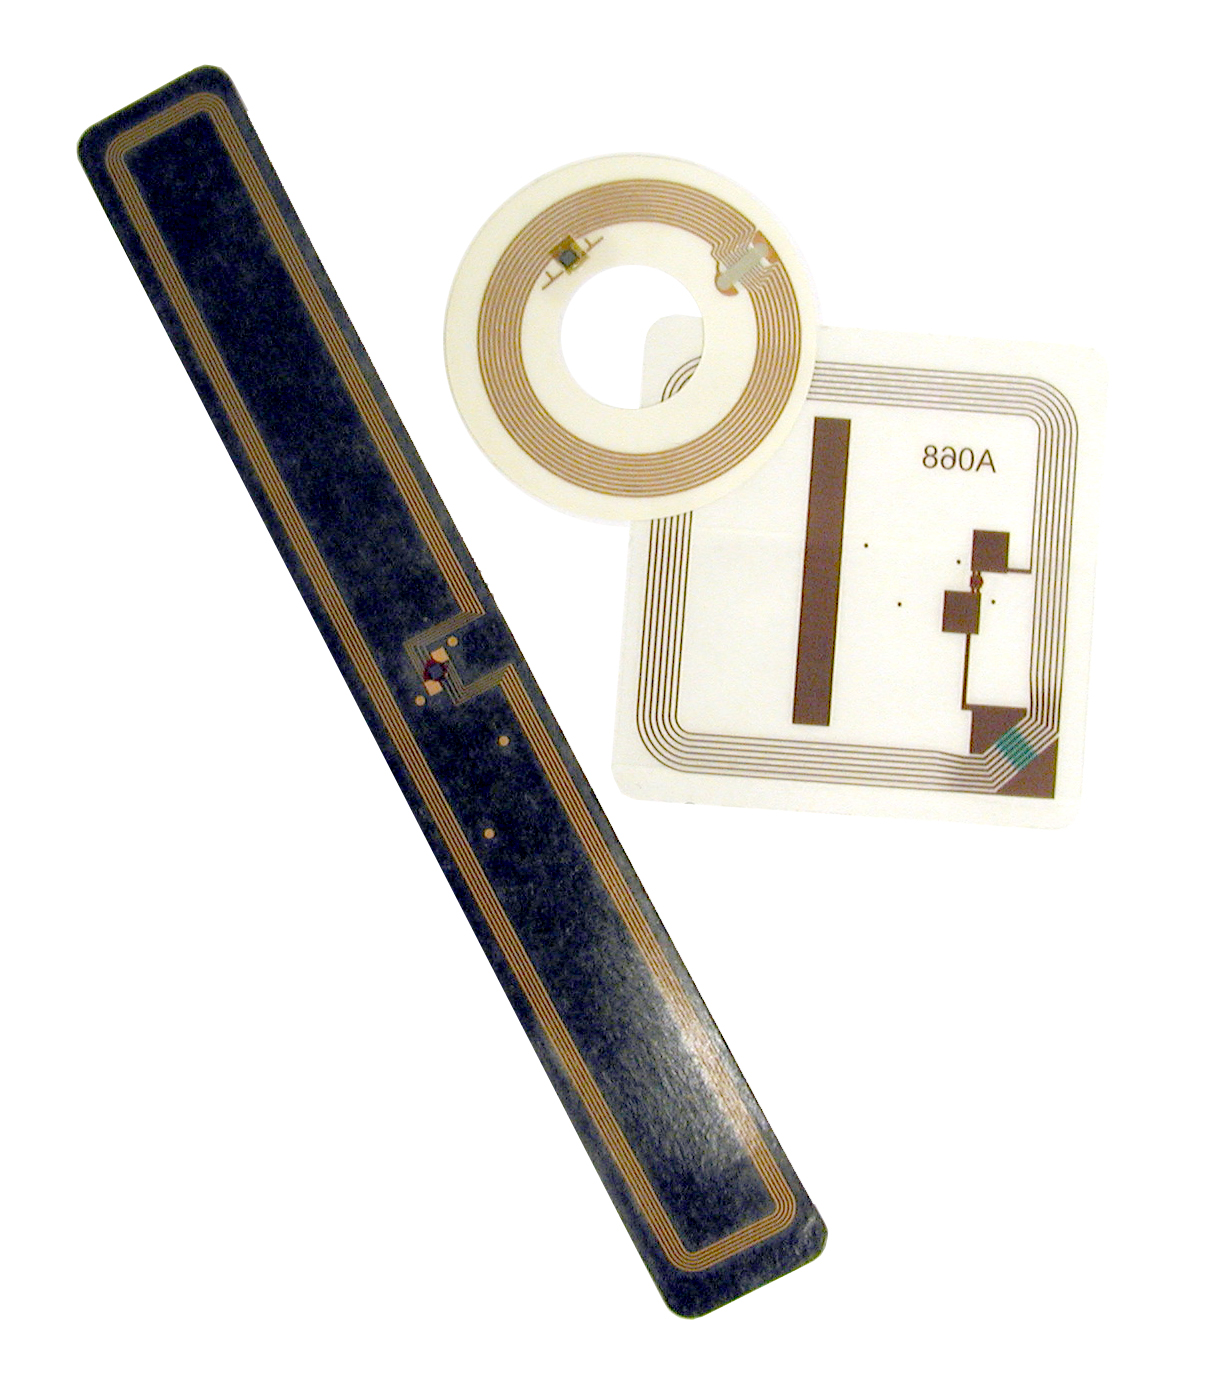
\includegraphics[width=0.2\textwidth]{img/RFID_Tags.jpg}
\caption{Verschiedene RFID Transponder \footnote{https://upload.wikimedia.org/wikipedia/commons/e/e3/RFID\_Tags.jpg}}
\end{figure}
\end{frame}


\section{Grundlagen}
\begin{frame}
\frametitle{Grundlagen}
\begin{itemize}
	\item Lesegerät liest Daten aus einem Transponder
	\item Transponder gibt es in vielen Größen und Formen
	\item Grundlegender Aufbau eines Transponders:
	\begin{itemize}
		\item Spulenförmige Antenne
		\item Schaltkreise zum Senden/Empfangen
		\item Speicher
	\end{itemize}
	
	\item Aktive/Passive Transponder
	\begin{itemize}
		\item Aktiver Transponder $\rightarrow$ eigene Spannungsquelle
		\item Passiver Transponder $\rightarrow$ keine eigene Spannungsquelle
	\end{itemize}
\end{itemize}
\end{frame}


\begin{frame}
\frametitle{Grundlegendes Kommunikationsschema}

\begin{enumerate}
	\item Lesegerät induziert Spannung und Taktfrequenz
	\item Lesegerät sendet Anfrage an Transponder
	\item Transponder übermittelt entsprechende Daten
\end{enumerate}

\begin{figure}
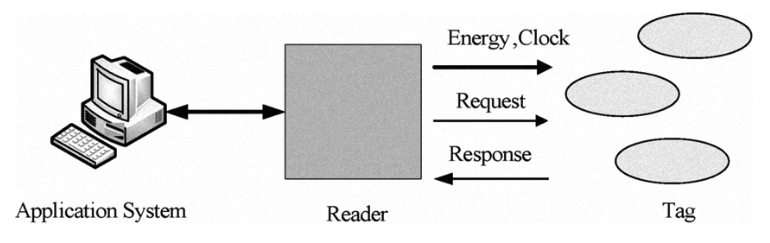
\includegraphics[width=0.7\textwidth]{img/kommunikation.png}
\caption{Kommunikationsschema \footnote{Chih-Yung Chen, Chien-Ping Kuo and Fang-Yuan Chien, "An exploration of RFID information security and privacy"}}
\end{figure}
\end{frame}

\section{Schwachstellen}
\begin{frame}
\frametitle{}

\end{frame}

\section{Angriffe auf Sicherheit und Privatsphäre}
\begin{frame}
\frametitle{}

\end{frame}

\section{Sicherheitsmaßnahmen}
\begin{frame}
\frametitle{}

\end{frame}

\section{Durchführbarkeit Angriffe}
\begin{frame}
\frametitle{}

\end{frame}

\section{Fazit}
\begin{frame}
\frametitle{}

\end{frame}


\end{document}